\begin{enumerate}
\item In \figref{fig:Fig_1}, two concentric circles with centre $O$, have radii $21 cm$ and $42 cm$. If $\angle AOB = 60\degree$, find the area of the shaded region.
\begin{figure}[H]
    \centering
    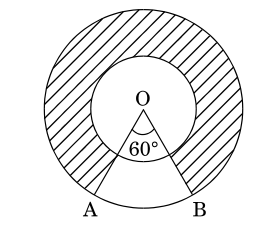
\includegraphics[width=\columnwidth]{figs/geo.png}
    \caption{Circle $AOB$ }
    \label{fig:Fig_1}
\end{figure}

\item A moving boat is observed from the top of a $150m$ high cliff moving away from the cliff. The angle of depression of the boat changes from $60\degree$ to $45\degree$ in $2$ minutes. Find the speed of the boat in m/min.

\item There are two poles, one each on either bank of a river just opposite to each other. One pole is $60m$ high. From the top of this pole, the angle of depression of the top and foot of the other pole are $30\degree$ and $60\degree$respectively. Find the width of the river and height of the other pole.

\item A cone of height $24 cm$ and radius of base $6 cm$ is made up of modelling clay. A child reshapes it in the form of a sphere. Find the radius of the sphere and hence find the surface area of this sphere.

\item A farmer connects a pipe of internal diameter $20 cm$ from a canal into a cylindrical tank in his field which is $10 m$ in diameter and $2 m$ deep. If water flows through the pipe at the rate of $3 km/hr$, in how much time will the tank be filled ?

\item Find the dimensions of a rectangular park whose perimeter is $60 m$ and area $200 m^2$.

\item A container opened at the top and made up of a metal sheet, is in the form of a frustum of a cone of height $16$ cm with radii of its lower and upper ends as $8$ cm and $20$ cm respectively. Find the cost of milk which can completely fill the container, at the rate of \rupee $50$ per litre. Also find the cost of metal sheet used to make the container, if it costs \rupee$ 10$ per $100 cm^2$. Take$\brak{\pi = 3.14}$

\end{enumerate}

